\section{Research that corrects its interpretation}
\label{section:research-that-can-inspect-its-own-results}

These mechanisms matter most when a result needs to be questioned rather than merely stored. Eigen's campaign on the SuperARC benchmark followed that path: an attractive score prompted closer examination of what the score measured. Its strongest scientific product was the resulting correction.

The original benchmark starts from an algorithmic-information idea: a compact executable account of data can express structure that literal reproduction does not. A program has consequences. It can be run, compared with a target and challenged on new inputs. SuperARC turns that motivation into several finite tests, including sequence reconstruction and prediction. Those are distinct tasks: reproducing a supplied finite prefix does not establish its unseen continuation.\footnote{Hern\'andez-Espinosa et al., \emph{SuperARC: a test for artificial superintelligence based on compressed modelling, recursive prediction and problem complexity}, Nature Communications 17,4885 (2026), \href{https://doi.org/10.1038/s41467-026-73289-5}{doi:10.1038/s41467-026-73289-5}.}~\cite{HernndezEspinosa2026c672f1}

For its reconstruction score, correct answers are divided into non-print/non-ordinal, ordinal and print categories. If their fractions are $\rho_1,\rho_2,\rho_3$, the score is
\begin{equation}
 \phi=\rho_1\delta_1+0.1\rho_2\delta_2+0.01\rho_3\delta_3.
 \label{eq:superarc-score}
\end{equation}
Within each category, $\delta_k$ is a harmonic mean of $\tanh[\mathrm{nBDM}(\mathrm{target})/\mathrm{nBDM}(\mathrm{answer})]$. Normalised block decomposition complexity, nBDM, is a finite operational approximation inspired by algorithmic information theory. The category weights build a preference for generative-looking answers into the instrument. Changing an answer's category can change its contribution by a factor of ten or a hundred without changing execution correctness.

The Eigen SuperARC campaign  generated answers to 100 twelve-term binary sequences using a bare arm, an iterative loop and an execute/fix comparison arm. All three recorded correct outcomes on every target under their respective checking routes. Their answer forms differed sharply: the bare arm mostly printed the sequence, while the two active arms mostly produced generative-looking expressions. Figure~\ref{fig:dd-superarc-controls} shows how those categories and the subsequent format controls affect the score.
\begin{figure}[htbp]
\centering
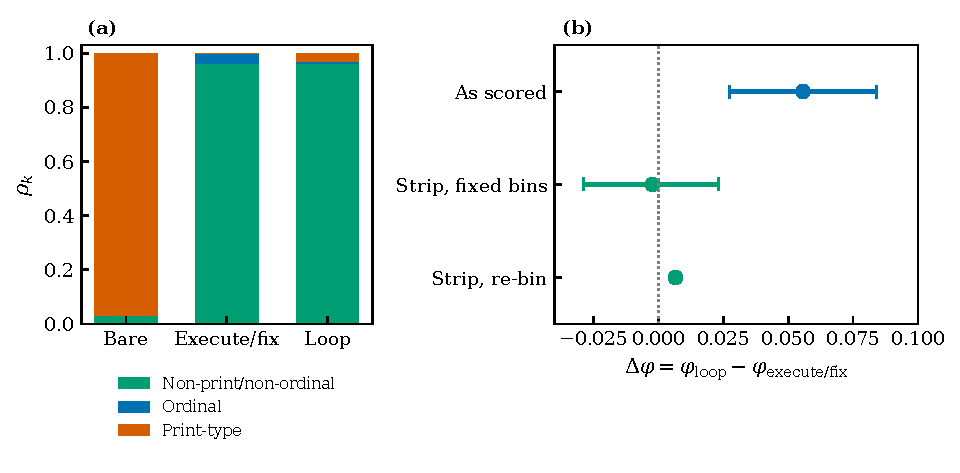
\includegraphics[width=\linewidth]{figures/portable-run-b69220b3a27348ad.result/dd-superarc-controls.pdf}
\caption{The recorded Eigen campaign on the SuperARC reconstruction task. (a) Fractions $\rho_k$ in each correct-answer category for $N=100$ twelve-term binary targets. All arms recorded correct outcomes through their distinct checking routes. (b) Loop-minus-execute/fix score difference $\Delta\phi$. Stripping commentary with categories fixed removes the positive separation. Bars are the archived 95\% paired-bootstrap intervals at resample size 100, seed 20260804 and 100 resamples. No interval was reported for the re-binned point. Formula-text scoring, program correctness and unequal search protocols prevent a causal recursion claim.}
\label{fig:dd-superarc-controls}
\end{figure}

The actual scored object requires care. Complexity was computed from formula text, not simply from the executable program retained beside it. Bare-arm correctness used scorer-side translation. The other arms used their banked programs, with an additional translation cross-check that did not always agree or succeed. This distinction matters because the scoring representation and the executable witness can otherwise appear to be the same object. The campaign preserved enough of both to expose the mismatch.

The adversarial follow-up found a direct confound. Commentary was much more common in loop answers, and the normalised text-complexity calculation could reward that extra text without adding generative information. Stripping commentary while holding answer categories fixed removes the positive loop-minus-execute/fix separation, as Figure~\ref{fig:dd-superarc-controls} shows. Reclassifying the stripped answers is a different protocol and gives a different point estimate. The apparent advantage was therefore sensitive to the representation being scored.

This correction is the campaign's most informative outcome. The system built an instrument, generated and executed candidates, preserved a frozen result, tested competing explanations and revised the interpretation. Unequal prompts and search access still require a controlled follow-up to isolate the effect of execution feedback. The demonstrated capacity is sustained research that leaves its conclusions open to inspection and correction.

The same process can be applied to the system's own explanation. A book describing the present research environment was written and revised using that environment: The Living System Guide . It explains the objects, tools, human decisions and recoverable work described above. Writing it therefore tested whether the system could use its own evidence to make its operation clearer.

One example concerned the effect of changing a source. Several claims used that source, and a further conclusion drew those claims together. The book's diagram needed to distinguish a change in the supporting material from a change in the conclusion's actual wording. Inspection of the implemented behaviour exposed where the explanation blurred those two things, and the caption was corrected. The useful outcome was a clearer account of when a reader should reconsider a conclusion even though its sentence has not changed.

The book also had to work for someone who had not built the system. An independent reader identified passages and figures that were difficult to follow. Those findings led to revisions, a rebuilt book and a focused reread. That cycle connects a technical construction to a usable explanation: the reader's difficulty becomes a concrete revision, whose source and rendered outcome remain inspectable.

A larger theoretical argument tests a different use of the same infrastructure. Foundations of Synthetics , the work from which the retained-state, residual and refinement constructions in this account were drawn, develops its argument through linked derivations, finite examples and explanatory figures. Those pieces retain their claims, evidence and revision history, so they can be extended and inspected separately while the manuscript explains how they fit together. The demonstration is the construction and maintenance of a connected argument, alongside the individual mathematical results it contains.

The three demonstrations now form a progression: investigate a benchmark, improve the system's own explanation, and build a larger theoretical account from inspectable parts. Each leaves material that can support the next piece of work. This is the practical basis of guided self-improvement: an agent helps build and test a capability, while an author sets its direction and acceptance conditions. To make that capacity useful beyond these projects, the same objects and operations must become understandable and extensible to another developer.

